\section{Definition classes (forslag accepteres)}
In order to get a good interpretation of the aspects of the \cube{}, then the different positions, faces and moves must be defined in an easy accessible way for both humans and computers. We solved this by defining three enumeration classes. 

One containing the possible positions and one defining the possible moves and one defining the faces.

\subsection{Moves}
\label{sub:moves}
The enumeration class that contains all possible moves actually contains a property for each button in the GUI. Confusing as this might seem it actually saved a lot of time and worked quite well. Of course the permute method of the cube can be called with a button which is not a move and cause an error. This is not a robust program but a proof-of-concept. 
The moves are named from a human perspective where the prime (\m{'}) is replaces by a ``P'', e.g. \m{U'} is \vr{UP}.

\subsection{Faces}
\label{sub:cubeFaces}
The different types of faces is well know by humans by its color.
But in the program we do not define the faces by color but by its \facelet{} attribute. 
The faces and the \facelet{}s are divided into primary, secondary and tertiary faces. 
Each consist of two opposite faces. Therefore each face is known by its type and a number 0 or 1 (see figure \ref{fig:faceRanking}) e. g. the up face (the white face) is know in the program as \textit{primary\_0}.
Its opposite, the yellow face, is know as \textit{primary\_1}. 

\begin{figure}[htbp]
	\centering
		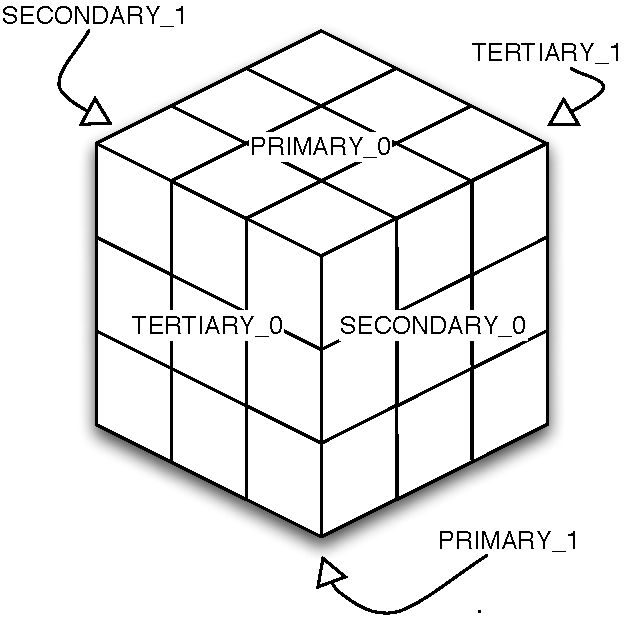
\includegraphics[scale=0.5]{input/pics/faceRanking.pdf}
	\caption{The different faces of a cube. The colors can be defined as whatever one wants.}
	\label{fig:faceRanking}
\end{figure}


\subsection{Positions}
The different positions are defined where the faces are based. There are two types of positions; corners and edges.
An edge position could be named \vr{P1S0}; which means \textit{primary\_1} and \textit{secondary\_0}.
In human terms this will be the down front edge.
Corners have three faces and the corner immediately to the right of the edge would be \vr{P1S0T1}, which refers to the corner on the \textit{primary\_1}, \textit{secondary\_0}, and \textit{tertiary\_1} faces.
